\documentclass[main.tex]{subfiles}
\begin{document}


\chapter{Search for $\beta\beta$ decay of $^{\text{116}}$Cd into the excited states of $^{\text{116}}$Sn}



\begin{flushright}
\textit{blablab lablab labla labla labla labla labla lablalabla \\ 
labla lablala labla labla lablabla labla}\\
Author.
\end{flushright}


\bigskip


\NI The aim of this analysis is to measure or set a limit on the half-life of the 2$\nu\beta\beta$ and 0$\nu\beta\beta$ decays of \Cd~via the excited states of \Sn.

\section{The \texorpdfstring{\Cd}~ sector in NEMO-3}
\label{sec:CdSectorInNEMO3}


\NI In NEMO-3 detector, a total mass of 440~g of cadmium were placed in sector 18. The average enrichment of \Cd~was (93.2~$\pm$~0.2)\%~\cite{NEMO-3-detector} which represents an effective mass of (410~$\pm$~1)~g~of~\Cd. The enrichment have been realized by the centrifugation separation method. Despite the good yield of this technique, smaller amounts of other isotopes are still present in the sample as summarized in Table~\ref{IsotopeCdTable}. Part of the sample (152~g) was previously measured with the NEMO-2 prototype~\cite{ObservationCd116NEMO-2}.  


\bigskip


\NI The cadmium has been divided in 7~strips of about 2423~cm long and about 65~cm wide. Each strip was made of one or more smaller pieces which were glued together with Araldite~AW~106 and a hardener~HV953V. Two 12-$\mu$m mylar films surrounded the entire strip to provide a mechanical strenght. The mylar films were glued using Araldite~2020/A~XW~3961 and Araldite~2020/B~XW~3972.


\begin{table}[h!]
\begin{center}
\begin{tabular}{c|c|c}
\toprule
Isotope & Mass fraction & Mass (g) \\
\midrule
116   & 0.932   & 410.08 \\[0.05cm]
114   & 0.03228 & 14.20  \\[0.05cm]
113   & 0.00885 & 3.90   \\[0.05cm]
112   & 0.01544 & 6.79   \\[0.05cm]
111   & 0.00535 & 2.35   \\[0.05cm]
110   & 0.00468 & 2.06   \\[0.05cm]
108   & 0.00032 & 0.14   \\[0.05cm]
106   & 0.00038 & 0.17   \\[0.05cm]
Total & 0.999   & 439.69 \\[0.05cm]
\bottomrule
\end{tabular}
\end{center}
\label{IsotopeCdTable}
\caption{Isotopes present in the 440~g of Cd sample placed in NEMO-3 detector. The total mass of \Cd~is (410~$\pm$~1)~g which takes into account the error on the enrichment yield of 0.2\%.}
\end{table}


\bigskip


\NI To ensure a good bound with the glue, the mylar sheets were perforated of microscopic holes (around 0.4 $\mu$m in diameter). The perforation has been realized at the Joint Institute for Nuclear Reaserch (JINR, Dubna, Russia) by irradiating the mylar with a $^{\text{84}}$Kr ion beam of 3~MeV/nucleon and a luminosity of 5~$\times$~10$^{\text{11}}$ ions/s. The mylar was chemically etched with NaOH at 70$^{\circ}$~C, washed with water and 1~\% of acetic acid. Finally, the film was dried with hot air. All the materials entering in the process of the backing film have been selected for their radio-purity and have been measured with High Purity Germanium detector at LSM.


\bigskip


\NI Each strips was connected to their neighboring strips with glue (Araldine~AW106). A schematic view of the~7~cadmium foils in sector~18 is shown in~Figure~\ref{CdFoil}. After the installation, some gaps ranging from 2~mm to 4~mm between some parts of the strips have been observed. The source shape is not strictly cylindrical as shown in the top section of~Figure~\ref{CdFoil}. It was also found that straining of the strips was small due to the softness of the cadmium metal~\cite{SoftnessCdMetal}. 


\bigskip


\begin{figure}[h!]
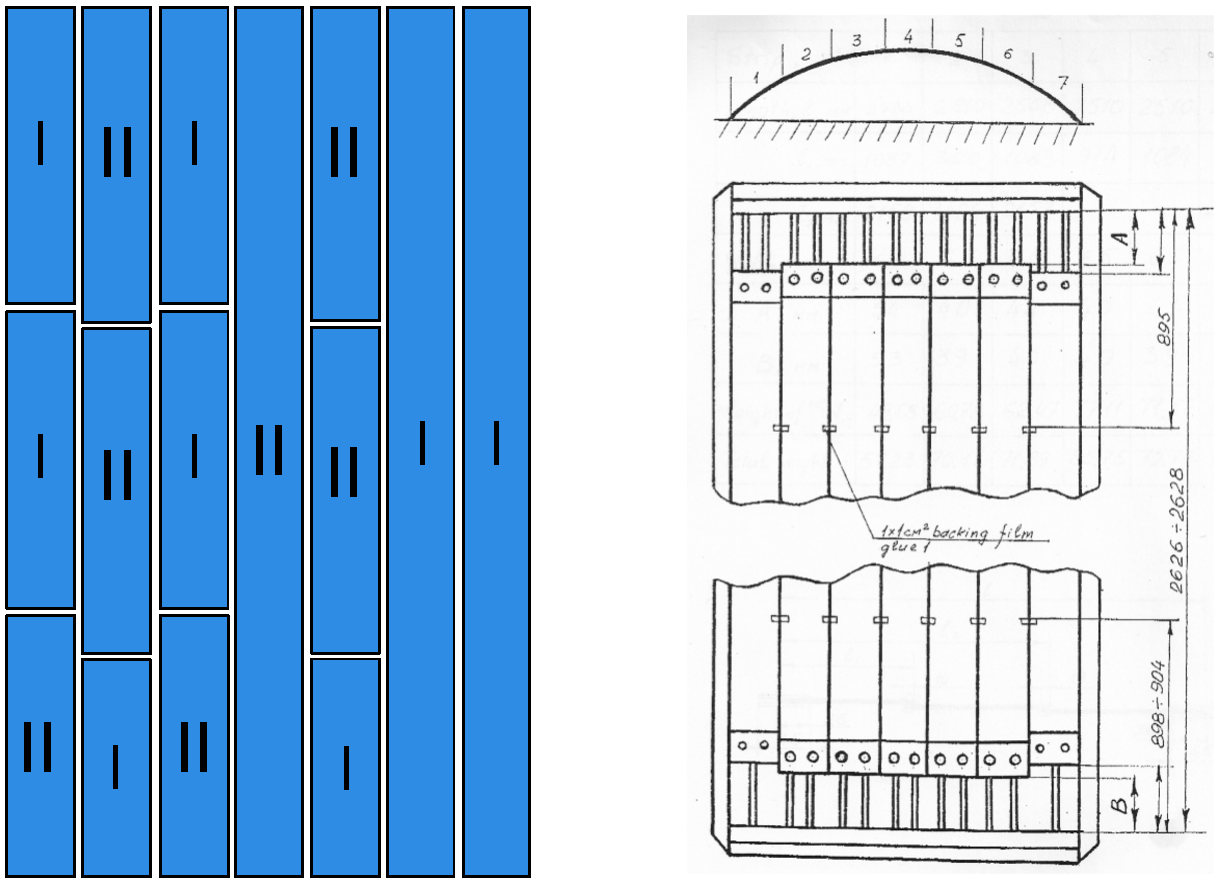
\includegraphics[height=7.5cm]{pictures/Chap6/schemaFoil_v2.pdf}
\centering
\caption{Left : Schematic view of the sector 18. The 7 cadmium foils are divided in smaller pieces and glued together. The labels I and II correspond to the different \Cd~productions. Right : Drawing of the strips of cadmium showing the plexiglass clips that attach the foil to the support structure. The small pieces of backing film used to join the individual strips to one another.}
\label{CdFoil}
\end{figure}


\NI Before to be introduced in the detector, the radioactive contaminations of the cadmium foils have been measured thanks to High Purity Germanium detector (HPGe). The results of the different contaminations are summarized in Table \ref{TableContaminationMeasurements}.


\bigskip


\begin{table}[h!]
\begin{center}
\begin{tabular}{c|c|c|c|c|c|c|c|c}
   \toprule
   Source  & Mass [g] & Exposure [h] &\multicolumn{6}{c|}{Activity [mBq/kg]} \\
   \midrule[0.05cm]
           &          &              & $^{\text{40}}$K &  $^{\text{235}}$U &  $^{\text{234}}$Th & $^{\text{214}}$Bi  & $^{\text{228}}$Ac & $^{\text{232}}$Tl \\[0.1cm]
   Type I  & 257      & 778          & < 13     & < 0.5      & < 12        & < 1.5                  & < 2        & < 0.5 \\
   Type II & 299      & 368          & < 20     & < 1        & < 56        & < 1.7                  & < 4        & < 0.83 \\
   \bottomrule
\end{tabular}
\caption{Measurements of the cadmium source foils (including mylar support) realized with HPGe detector.}
\label{TableContaminationMeasurements}
\end{center}
\end{table}


\FloatBarrier



\section{Excited states of \texorpdfstring{$^{\text{116}}$}~Sn}
\label{sec:ESCd}

\NI The search for the 2$\nu\beta\beta$ and 0$\nu\beta\beta$ decays to the ground state have been investigated with the full statistic of NEMO-3~\cite{Arnold2016bed}. In theory, the $\beta \beta$ decays can also occur through the excited states of the daughter nucleus. Due to smaller space phases these decays to the excited states are even rarer than the decay to the fundamental state but some of them have already been observed for $^{\text{100}}$Mo and $^{\text{150}}$Nd nuclei~\cite{Barabash2010ie}. Concerning the \Cd, the $\beta \beta$ decays via the excited have never been found. The results of this analysis will lead to the first values or limits put with the NEMO-3 data on these processes.


\bigskip


\NI The searches for $\beta \beta$ decays through the excited states is mainly motivated by a better understanding of the nuclear structures. The measurement of the decay rate brings informations about the squared effective axial-vector coupling constant and nuclear matrix elements which are sensitive to nuclear-spin isospin correlations. The decays via the excited states is also interesting to study the 0$\nu\beta\beta$ mechanism. They can provide possibilities to distinguish between the various 0$\nu\beta\beta$ mechanisms by studying the different branching ratios of 0$\nu\beta\beta$ of excited states and ground state~\cite{TheoryOfNeutrinolessDBD}.


\bigskip


\NI The simplified schema of the \Cd~decay to \Sn~is shown in Figure \ref{SchemaExcitedState}. Only the 2 first excited states are considered at 1294 keV (2$^+$) and at 1757 keV (0$^+$). These two excited states will be studied in case of 2$\nu\beta\beta$ and 0$\nu\beta\beta$. The label and the description of each case are given below :



\begin{itemize}
\item \textbf{(0$^+$) 2$\nu$} : The signature of this decay is the simultaneous emission of 2~electrons and 2~photons. The Q$_{\beta \beta}$ of the electron energy spectrum is 1048 keV. The photon energy spectrum is very characteristic with the two peaks at 463 keV and 1294 keV.

\item \textbf{(0$^+$) 0$\nu$} : The signature of this decay is the simultaneous emission of 2~electrons and 2~photons. As no neutrino is emitted, the electron energy sum spectrum is peaked at 1048 keV. The photon energy spectrum is the same than in (0$^+$) 2$\nu$.

\item \textbf{(2$^+$) 2$\nu$} : The signature of this decay is the simultaneous emission of 2~electrons and 1~photon. The Q$_{\beta \beta}$ of the electron energy spectrum is 1511 keV. The gamma energy spectrum is characterized by a peak at 1294 keV.

\item \textbf{(2$^+$) 0$\nu$} : The signature of this decay is the simultaneous emission of 2~electrons and 1~photon. The electron energy sum spectrum is caracterized by a peak at 1511 keV. The photon energy spectrum is the same than in (2$^+$) 2$\nu$.
\end{itemize}



\begin{figure} [h!]
\begin{center}
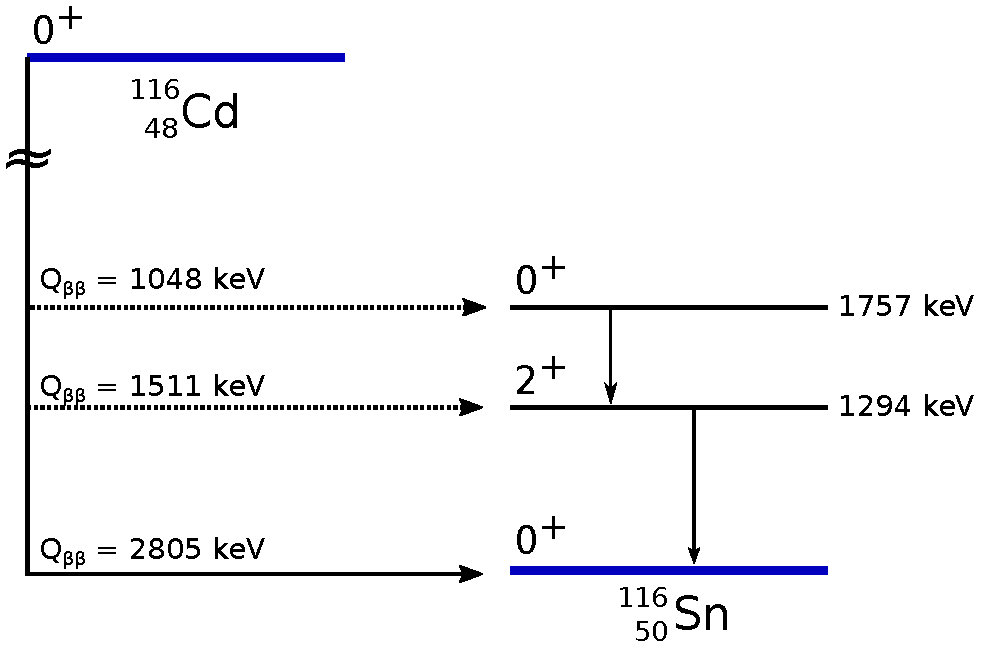
\includegraphics[scale=0.60]{pictures/Chap6/SchemaCdExcitedState.pdf}
\end{center}
\caption{Schema of the two main excited of $^{\text{116}}$Sn. The excited state 0$^+$ (1757 keV) corresponds to the emission of two electrons with a Q$_{\beta\beta}$~=~1048~keV and two photons at~1294~keV and 463~keV. The excited state 2$^+$~(1294~keV) corresponds to the emission of two electrons with a Q$_{\beta\beta}$~=~1511~keV and one photon at~1294~keV. In case of 2$\nu\beta\beta$ these decays are accompagnied by two neutrinos.}
\label{SchemaExcitedState}
\end{figure}



\NI Theoretically, the decay probability to the excited states is proportionnal to (Q$_{\beta\beta}$ $-$ E$^*$)$^{\text{11}}$ in 2$\nu\beta\beta$ decay and to (Q$_{\beta\beta}$ $-$ E$^*$)$^{\text{5}}$ in 0$\nu\beta\beta$ decay, where Q$_{\beta\beta}$ is the total available energy and E$^*$ the energy of the excited state. It can be deduced that the decay to the excited state~2$^+$ is more likely than the decay via~0$^+$. Furthermore, as the detection efficiency of the electrons increases with the their energy, the decays via the excited state 2$^+$ seems easier to detect. One the other hand, the presence of 2 electrons and 1 photon inside the detector is more reproducible by the background than the presence of 2 electrons and 2 photons. In any case, the detection efficency of the two electrons and one or more photons will be very low. It explains why the search for decays via the excited states is very challenging.


\bigskip


\NI Historically, the first observation of the \Cd~ 2$\nu\beta\beta$ decay was reported in 1995 by three independent experiments : NEMO-2~\cite{Barabash2010ie}, Elegant-V~\cite{ElegantV-1} and at the Solotvina Underground laboratory\cite{Aurora}. NEMO-2 was installed at LSM and took data during ten months with a enriched cadmium source surrounded by tracking chamber and plastic scintillator calorimeter. The half-life of 2$\nu\beta\beta$ was measured to be T$_{\text{1}/\text{2}}^{\text{2}\nu}$~=~(3.75 $\pm$ 0.35 (stat) $\pm$ 0.21~(syst)~)~$\times$~10$^{\text{19}}$~y. Limit at 90\% C.L on the \Cd~half-lives of T$_{\text{1}/\text{2}}^{\text{0}\nu}$~>~5.0~$\times$~10$^{\text{21}}$ y for 0$\nu\beta\beta$ decay were obtained with an exposure of 0.11~kg$\times$y. In the same time, ELEGANT-V reported the results of the double beta decay using natural and enriched cadmium foils sandwiched between drift chambers and plastic scintillators. Sodium iodide scintillators was used to enhance background rejection. The half-life have been measured to be T$_{\text{1}/\text{2}}^{\text{2}\nu}$~=~2.6 $^{+\text{0.9}}_{-\text{0.5}}$~$\times$~10$^{\text{19}}$~y with an exposure of 0.02~kg$\times$y. A lower limit on the 0$\nu\beta\beta$ was set to T$_{\text{1}/\text{2}}^{\text{0}\nu}$ > 2.9~$\times$~10$^{\text{21}}$~y. These measurements are compatible with the results obtained with cadmium tungstate crystal scintillators at the Solotvina Underground Laboratory.  The half-life of 2$\nu\beta\beta$ was measured to be T$_{\text{1}/\text{2}}^{\text{2}\nu}$~=~2.7$^{+\text{0.5}}_{-\text{0.4}}$~$\times$~10$^{\text{19}}$~y. The lower limit on the half-life was set to T$_{\text{1}/\text{2}}^{\text{0}\nu}$~>~2.9~$\times$~10$^{\text{22}}$~y at 90\%C.L. 


\bigskip


\NI More recently the study of the \Cd~decay has continued mainly using CdWO$_{\text{4}}$ scintillator crystals. The Solotvina experiment reported the results obtained with 330 g of crystals for a total exposure  of 0.4~kg$\times$y~\cite{Solotvina}. The 2$\nu\beta\beta$ half-life corresponding to T$_{\text{1}/\text{2}}^{\text{2}\nu}$~=~[2.9 $\pm$ 0.06 (stat.) $^{+\text{0.4}}_{-\text{0.3}}$ (syst.)]~$\times$~10$^{\text{19}}$~y. Installed at the Gran Sasso Underground Laboratory, Aurora experiment investigate double beta decay of \Cd~ with 1.162~kg of crystal scintillators enriched to 82~\%~\cite{Aurora}. The half-life of 2$\nu\beta\beta$ was measured to be T$_{\text{1}/\text{2}}^{\text{2}\nu}$~=~[2.62 $\pm$ 0.14]~$\times$~10$^{\text{19}}$~y for the ground state. The lower limit on the half-life was set to T$_{\text{1}/\text{2}}^{\text{0}\nu}$~>~1.7~$\times$~10$^{\text{23}}$~y at 90\%~C.L. Aurora has also puts new limits concerning the decay of \Cd~via the excited state of \Sn. The main results obtained for 2$\nu\beta\beta$ and 0$\nu\beta\beta$ decays to the ground and the excited states are gathered in Table~\ref{TableSummaryResultsFS}.\textcolor{red}{mettre à jour et trouver les infos et les réfs}.



\begin{table}[h!]
\begin{center}
\begin{tabular}{c|c|c}
\toprule
Experiment &  Decays & T$_{\text{1}/\text{2}}$ half-life or limit [y] at 90 \% C.L\\[0.1cm]
\midrule[0.05cm]

\multirow{2}{*}{NEMO-2} & 2$\nu$ (g.s) & [3.75 $\pm$ 0.35 (stat.) $\pm$ 0.21 (syst.)]~$\times~$10$^{\text{19}}$\\[0.1cm]
                        & 0$\nu$ (g.s) & $>$ 5~$\times$~10$^{\text{22}}$ \\[0.1cm]
                                               
\midrule   
\multirow{2}{*}{NEMO-3} & 2$\nu$ (g.s) & [2.74 $\pm$ 0.04 (stat.) $\pm$ 0.18 (syst.)]~$\times$~10$^{\text{19}}$\\[0.1cm]
                        & 0$\nu$ (g.s) & $>$ 1.0~$\times$~10$^{\text{23}}$ \\[0.1cm]
                    
\midrule                        

\multirow{2}{*}{ELEGANT-V} & 2$\nu$ (g.s) & [2.6 $^{+\text{0.9}}_{-\text{0.5}}$]~$\times$~ 10$^{\text{19}}$\\[0.1cm]
                           & 0$\nu$ (g.s) & $>$ 2.9~$\times$~10$^{\text{22}}$ \\[0.1cm]
                        
                        
\midrule

\multirow{2}{*}{CdWO$_{4}$} & 2$\nu$ (g.s) & [2.7 $^{+\text{0.5}}_{-\text{0.4}}$~(stat.)~$^{+\text{0.9}}_{-\text{0.6}}$~(syst.)]~$\times$~10$^{\text{19}}$\\[0.1cm]
                           & 0$\nu$ (g.s) & $>$ 2.9~$\times$~10$^{\text{22}}$ \\[0.1cm]

\midrule
                           
                           
\multirow{2}{*}{Solotvina} & 2$\nu$ (g.s) & [2.9 $\pm$ 0.06 (stat.)~$^{+\text{0.4}}_{-\text{0.3}}$ (syst.)]~$\times$~10$^{\text{19}}$\\[0.1cm]
                           & 0$\nu$ (g.s) & $>$ 1.9~$\times$~10$^{\text{23}}$ \\[0.1cm]
                           

\midrule

\multirow{6}{*}{Aurora} & 2$\nu$ (g.s) & [2.62~$\pm$ 0.06~(stat.)~$\pm$~0.14~(syst.)]~$\times$~10$^{\text{19}}$\\[0.1cm]
                        & 2$\nu$ (0$^+$) & $>$ 9.0~$\times$~10$^{\text{20}}$\\[0.1cm]
                        & 2$\nu$ (2$^+$) & $>$ 1.0~$\times$~10$^{\text{21}}$\\[0.1cm]
                        & 0$\nu$ (g.s)   & $>$ 1.9~$\times$~10$^{\text{23}}$\\[0.1cm]
                        & 0$\nu$ (0$^+$) & $>$ 6.2~$\times$~10$^{\text{22}}$\\[0.1cm]
                        & 0$\nu$ (2$^+$) & $>$ 6.3~$\times$~10$^{\text{22}}$\\[0.1cm]
\bottomrule
\end{tabular}
\caption{Summary of results for the search for $\beta \beta 2\nu$ and $\beta \beta 0\nu$ decays to the fundamental and excited states.}
\label{TableSummaryResultsFS}
\end{center}
\end{table}


\FloatBarrier



\section{Background to the search for the excited states}


\NI The $\beta \beta$ decays to the excited states present very specific signatures : emission of  2 electrons accompanied by one or more photons. Moreover, the energies of these photons are very characteristic. Very few isotopes are able to reproduce this kind of signature. In NEMO-3, according its origin, the background is divided in two parts : 


\begin{itemize}
\item \textbf{Internal background} : regroups the backgrounds having their origin inside the source foil.
\item \textbf{External background} : regroups the backgrounds not coming from the source foil.
\end{itemize}


\subsection{Internal backgrounds}


\NI The internal background mainly provides from the presence of radioactive isotopes of the $^{\text{238}}$U and $^{\text{232}}$Th decay chains inside the source foil. The more troublesome are the isotopes with large Q$_\beta$ as $^{\text{208}}$Tl (Q$_\beta$~=~4.99~MeV) and $^{\text{214}}$Bi (Q$_{\beta}$~=~3.27 MeV). During their decays, they can induced 2-e like events thought three main processes :


\begin{itemize}
\item the electron emitted in $\beta$ decay can undergo a M\"oller scattering and create a second electron.
\item the $\beta$ emission can be accompanied by a second electron coming from the internal conversion of the daughter nucleus.
\item the $\beta$ decay is accompanied by a photon coming from the deexcitation of the daughter nucleus. A second electron is produced by Compton scattering of this photon.
\end{itemize} 


\NI These 2-e like events can be accompanied by one or more gamma emission(s) coming from Bremsstrahlung scattering or deexcitation of the  daughter nucleus after a decay. As the electron energy is not high (<~2~MeV), the creation of one photon is more likely that the creation of 2~photons. That is why the 2e1$\gamma$ channel is expected to be more polluted than the 2e2$\gamma$ channel by the background. The different mechanisms leading to 2-e like events accompanied with 2 photons at the origin of internal backgrounds are summarized in Figure~\ref{InternalBkgPicture}. The same mechanisms can also occur and be accompanied by only 1$\gamma$.



\begin{figure}[h!]
\centering
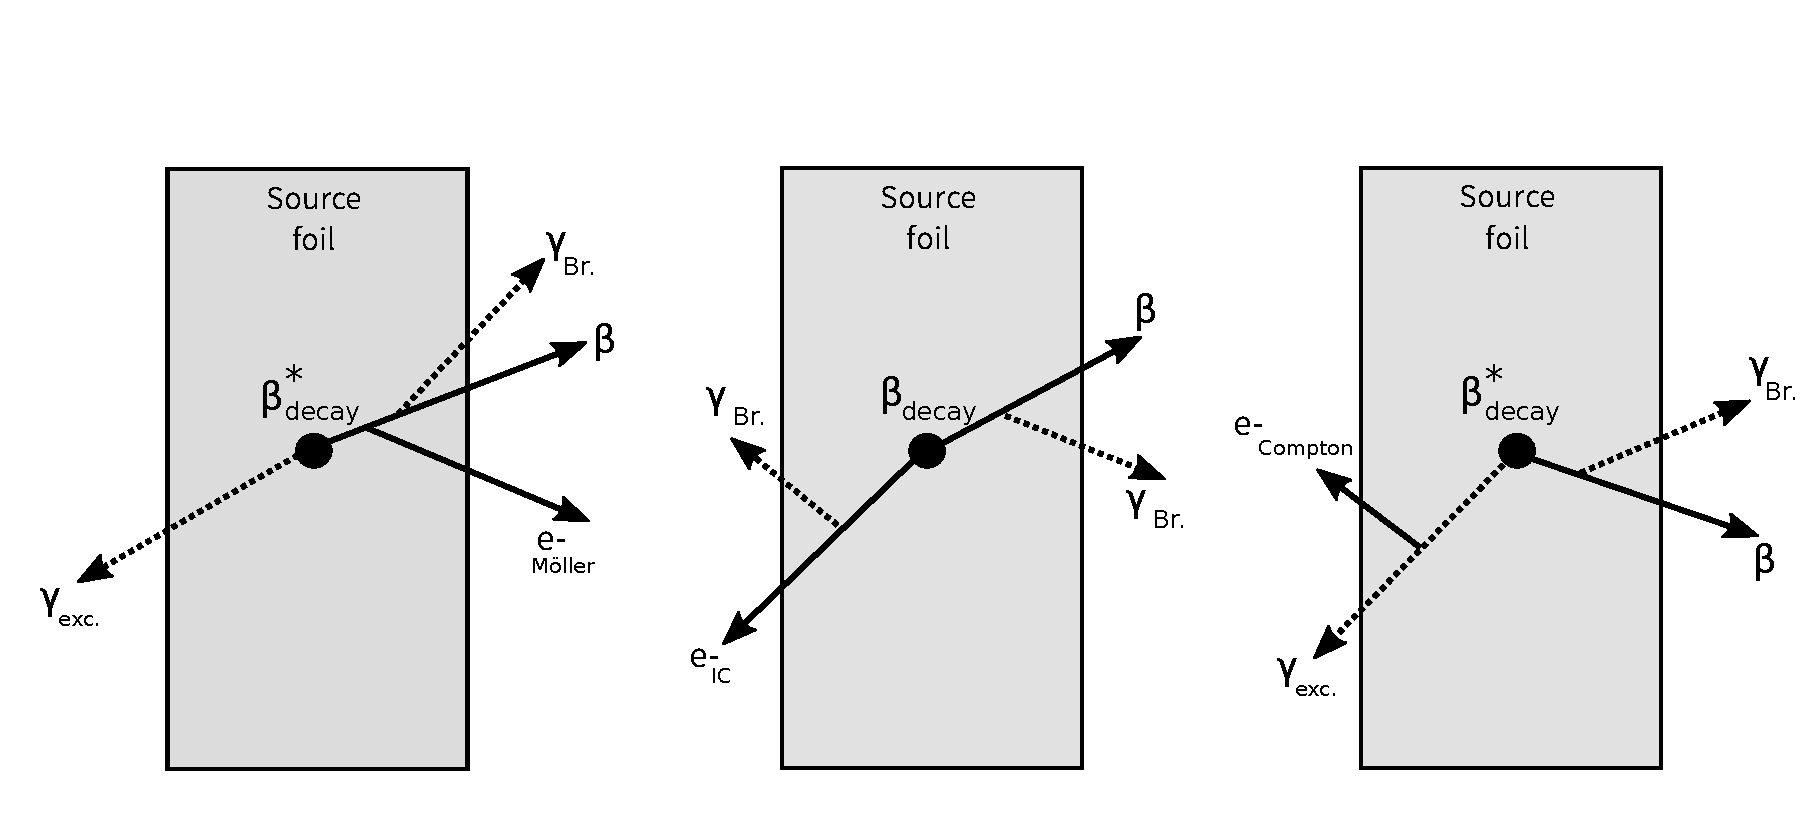
\includegraphics[scale=0.47]{pictures/Chap6/InternalBkg.pdf}
\label{InternalBkgPicture}
\caption{The different mecanisms leading to 2-e like events accompagnied with 2 photons at the origin of internal backgrounds. Left : a $\beta$-decay via excited state is followed by a M\"oller scaterring and Bremsstrahlung. Middle : $\beta$-decay with an internal conversion and 2 Bremsstrahlung effects. Right :  a $\beta$-decay via excited state is followed by a Compton scattering and Bremsstrahlung effect.}
\end{figure}



\NI The radioactive isotopes of the $^{\text{238}}$U and $^{\text{232}}$Th decay chains can be already present inside the initial source powder and not be entirely removed by the purification process. They can also be introduced latter during the source foil production, handling and mounting. Explaining why a great care was taken in the production and purification of the enriched materials, as well as during the source foil production and mounting.


\bigskip


\NI An other background to take into account when searching the excited state is the 2$\nu\beta\beta$ decay to the ground state. Each or both electrons of the 2$\nu\beta\beta$ decay can undergo a Bremsstrahlung scattering and mimic 2e1$\gamma$ or 2e2$\gamma$ events. The 2$\nu\beta\beta$ decay also constitutes an irreducible background for the search of 0$\nu\beta\beta$ decay. In the region where a signal of 0$\nu\beta\beta$ is expected some events of 2$\nu\beta\beta$ decay can be present. This contribution strongly depends of the 2$\nu\beta\beta$ half-life and the energy resolution of the detector.


\FloatBarrier


\subsection{External backgrounds}\label{sec:externalBkg}


\NI The presence of radioactive elements as radon and thoron inside the detector constitutes one of the main important external background component. These gases are released by the rock walls of the laboratory and are highly diffusive. They can enter inside the detector by tiny gaps between sectors or though gas pipe joints. The decays of these progeny produced photons and electrons. If such a decay occurs close to the source foil it is indistinguishable from an 2e events.


\bigskip


\NI The second important contribution of the external background is the interaction of photons with the source foil. These photons provide from different origins. A part of them is produced by neutron interactions in the shielding of the detector. They also come from radon in the air surrounding the detector. An other source of photon is the rock walls of the laboratory. The last contribution is the radioactive isotopes present in the detector. For example, despite a drastic selection, some traces of $^{\text{40}}$K, $^{\text{214}}$Bi and $^{\text{208}}$Tl have been found in the glass of the PMTs. The three mains mechanisms able to reproduce the 2e topology from an external photon are :   


\begin{itemize}
\item the $\gamma$ hitting the source foil create a pair (e$^+$e$^-$). Due to a bad a reconstruction of the track curvature of the e$^+$ is identified as an e$^-$.
\item the $\gamma$ hitting the source foil undergo a double Compton scattering.
\item the $\gamma$ hitting the source foil undergo a Compton scattering. A second electron is created in a M\"oller scattering of the emitted electron.
\end{itemize} 


\NI As in internal background, theses mecanisms can be accompagnied by one or more photons. The Figure \ref{ExternalBkgPicture}  summarizes the different processes. The $^{\text{210}}$Bi decay is also a possible source of background.



\begin{figure}[h!]
\begin{center}
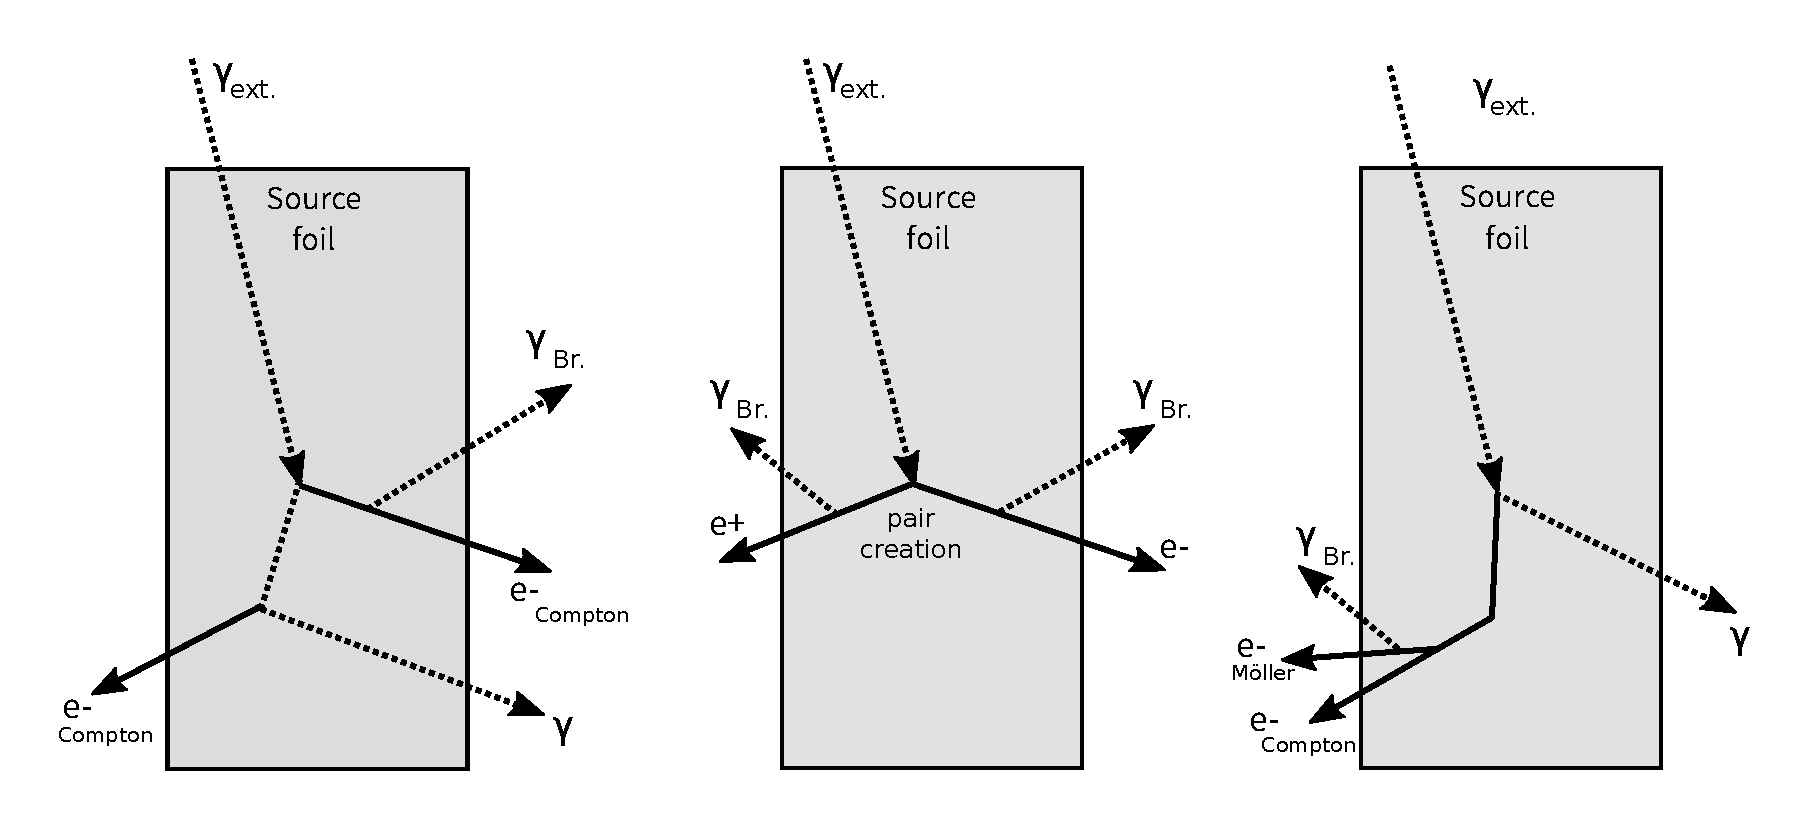
\includegraphics[scale=0.47]{pictures/Chap6/ExternalBkg.pdf}
\end{center}
\caption{Mechanisms leading to 2-e like events accompanied with 2 photons coming from an external $\gamma$. Left : the external $\gamma$ undergoes a double Compton scattering accompanied of Bremsstrahlung effects. Middle : pair creation from the external $\gamma$ with Bremsstrahlung effects. The positron is identified as an electron due to a bad reconstruction. Right : Compton scattering of the external $\gamma$ followed by a M\"oller diffusion of the electron and a Bremsstrahlung.}
\label{ExternalBkgPicture}
\end{figure}


\FloatBarrier


\subsection{Background model}


\NI The background model used in this analysis have been developed for the analysis of $\beta\beta$ decay of \Cd~to the ground state~\cite{Arnold2016bed}. The strategy is to benefit of the NEMO-3 ability to reconstruct the topology of the events. The backgrounds can be measured through different channels. The considered channels and the contaminations they can measured are detailed below.  


\bigskip


\subsubsection{Different activity region in the \Cd~sector}

\NI In the 1e channel~(the events selection are described in section~\ref{sec:1echannel}), the vertex distribution lets appear a non uniformity in activity of the foil, three activity regions have been defined, an high activity region $\gtrsim$~200 events/bin, a medium activity region with [100;200] events/bin and a low activity region with $\lesssim$~100 events/bin. The high activity region observed for Sector~$<$~18.08 corresponds to the calibration tube. This area is not take into account in the analysis since no \Cd~foil is present here. The other high activities regions match with the links between the different strips which compose the foil as described in section~\ref{sec:CdSectorInNEMO3} and shown in Figure~\ref{CdFoil}. The excess of events observed in the high activity region probably provides from a contamination of single $\beta$-emitters. This suggestion is supported by the observation of any strong excess in 1e1$\gamma$ channel as shown in~Figure~\ref{CdSector1eChannel}. The small excess corresponding to the emission of Bremsstrahlung by the single $\beta$-emitter. Studies realized by the collaboration highlighted an excess of $^{\text{234m}}$Pa with respect to $^{\text{40}}$K and $^{\text{210}}$Bi and validated the hypothesis that the single $\beta$-emitter is the origin of the high activity region.


\begin{figure}[h!]
\centering
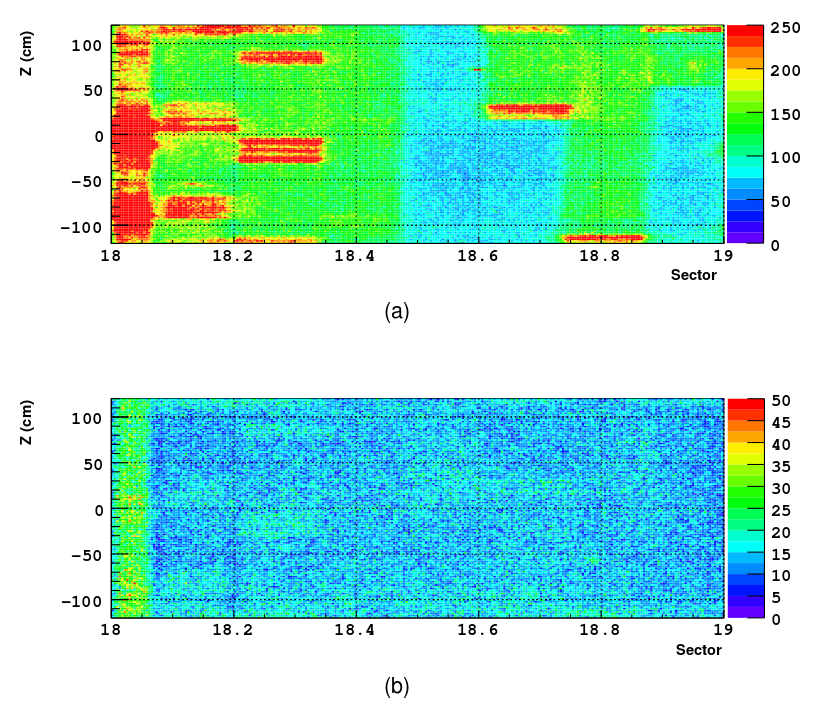
\includegraphics[scale=0.45]{pictures/Chap6/CdSector-1e-1e1g.png}
\label{CdSector1eChannel}
\caption{(a)~\Cd~sector in 1e channel. Blue region corresponds to the low activity region, the green region to medium activity. The high activity regions appear in red, these region are excluded of the analysis. (b)~\Cd~sector in 1e1$\gamma$ channel.}
\end{figure}


\bigskip


\NI The high activity regions are excluded from the analysis with simple rectangular cuts based on the number of events by bin. A total of 12 spots are defined as high activity regions which correspond to around 11\% of the \Cd~foil. The location of the removed area are presented in Table~\ref{Tab:HighActivityRegion}. 


\begin{table}
\centering
\begin{tabular}{c|c|c}
  & Z                 & Sector \\
\midrule
1  & [110.00 ; 120.00]   & [18.08 - 18.32] \\ [0.1cm]
2  & [114.00 ; 120.00]   & [18.61 - 18.75] \\ [0.1cm]
3  & [112.00 ; 120.00]   & [18.86 - 19.00] \\ [0.1cm]
4  & [76.00 ; 92.00]     & [18.21 - 18.35] \\ [0.1cm]
5  & [70.00 ; 73.00]     & [18.59 - 18.61] \\ [0.1cm]
6  & [0.00 ; 35.00]      & [18.08 - 18.23] \\ [0.1cm]
7  & [16.00 ; 34.00]     & [18.61 - 18.75] \\ [0.1cm]
8  & [-32.00 ; -3.00]    & [18.20 - 18.35] \\ [0.1cm]
9  & [-58.00 ; -52.00]   & [18.12 - 18.16] \\ [0.1cm]
10 & [-94.00 ; -64.00]   & [18.08 - 18.20] \\ [0.1cm]
11 & [-120.00 ; -112.00] & [18.14 - 18.35] \\ [0.1cm]
12 & [-120.00 ; -110.00] & [18.74 - 18.88] \\
\bottomrule
\end{tabular}
\caption{Location of the high activity region on the \Cd~foil in [Sector;Z] units. 12 regions are identified and excluded from the analysis which correspond to about 11 \% of the foil.}
\label{Tab:HighActivityRegion}
\end{table}


\FloatBarrier


\subsubsection{External backgrounds measurement}


\NI The model developed to estimate the external background is an effective model. Its aim is to provide an accurate description of the total external gamma flux in the detector region near the \Cd~foil. To measure the external backgrounds two channels are used : the one crossing electron channel (OCE) and the external electron-$\gamma$ (($\gamma$,e)$_{\text{Ext}}$) channel. As explained in Section~\ref{sec:externalBkg}, 


\bigskip


.  The total energy distribution is used in both channels to discriminate the different contributions and to perform the likelihood fit.



\begin{figure}[h!]
\centering
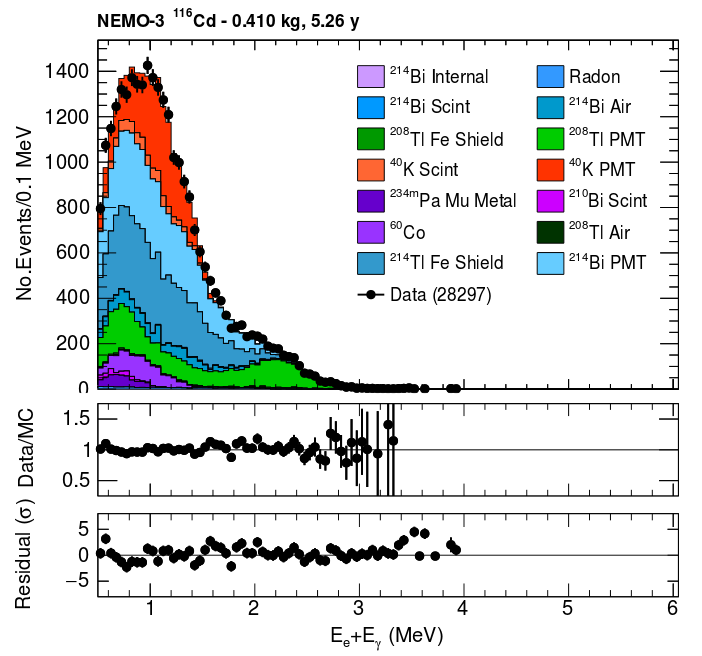
\includegraphics[scale=0.35]{pictures/Chap6/g-eChannelEtot.png}
\label{egChannel_Etot}
\caption{...}
\end{figure}


\begin{table}
\centering
\begin{tabular}{cc|c}
                                   &              &  Activity (Bq)   \\
\midrule
\multirow{2}{*}{$^{\text{40}}$K}   & PMT          & 1300  $\pm$ 45   \\
                                   & Scintillator & 19    $\pm$ 1    \\
\midrule
\multirow{4}{*}{$^{\text{210}}$Bi} & PMT          & 269   $\pm$ 47   \\
                                   & Air LSM (P1) & 600   $\pm$ 20   \\
                                   & Scintillator & 0.25  $\pm$ 0.03 \\
                                   & Fe Shield    & 10303 $\pm$ 2023 \\
\midrule
\multirow{3}{*}{$^{\text{208}}$Tl} & PMT          & 45.4   $\pm$ 1.4 \\
                                   & Air LSM (P1) & 14     $\pm$ 3   \\
                                   & Fe Shield    & 55     $\pm$ 50  \\
\midrule
$^{\text{210}}$Bi                  & Scintillator & 35     $\pm$ 4  \\
\midrule
$^{\text{60}}$Co                   & Tower + $\mu-$metal & 62 $\pm$ 13  \\
\midrule
$^{\text{234m}}$Pa                 & $\mu-$metal & 2655 $\pm$ 1180  \\
\bottomrule
\end{tabular}
\caption{External background activities measured in \Cd~sector.}
\label{TableOCE-activityMeasurement}
\end{table}


In this background model, the external contributions are measured only by using the data from the cadmium sector.


\FloatBarrier


\subsubsection{Internal $^{\text{214}}$Bi ($^{\text{222}}$Rn) measurement}


\NI As explained in Chap.~\ref{chap:Radon}, $^{\text{214}}$Bi the contamination is measured using the 1e1$\alpha$ channel. To be selected, an event has : 


\begin{itemize}
\item
\item
\item
\end{itemize}


\NI To verify the purity of this selection, the delayed time of the $\alpha$ is used. The time difference between the electron and the $\alpha$ matches with the half-life of $^{\text{214}}$Po of 164~$\mu$s as shown in Figure~\ref{1e1aChannel_alphaDelayTime}.


\bigskip


\NI The $\alpha$ track length is used to distinguish the different $^{\text{214}}$Bi contributions and to perform a likelihood fit. A total of 10 parameters are used corresponding to the different locations and phases. To take into account the diminution of the radon level after the installation of the anti-radon system, the $^{\text{214}}$Bi on the surface of the wires and foil are fitted separately (Phase 1 and Phase 2). The internal and mylar $^{\text{214}}$Bi contributions are not split according the phase as their activities are not expected to vary during the data taking. The results of the likelihood fit are summarized in~Table~\ref{Table1e1a-activityMeasurement}.


\begin{figure}[h!]
\centering
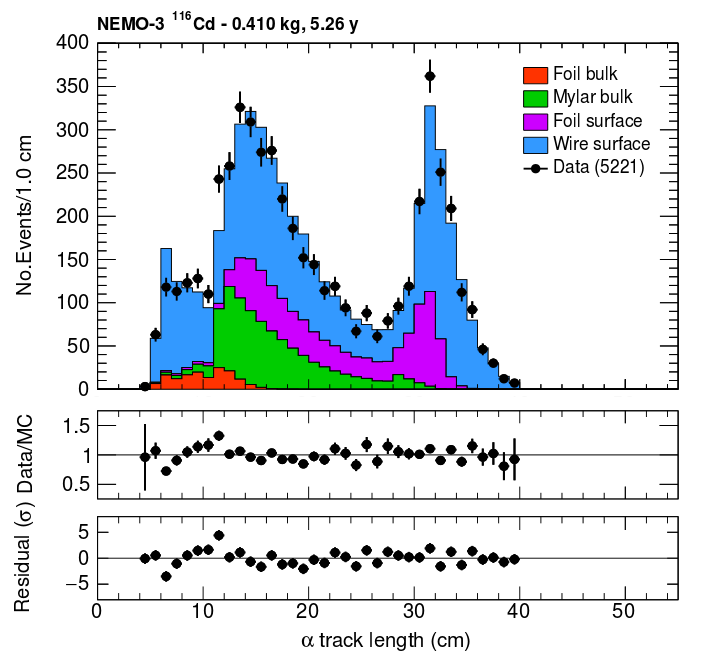
\includegraphics[scale=0.35]{pictures/Chap6/Bkg1e1aAlphaLength.png}
\label{1e1aChannel_alpphaLength}
\caption{Distribution of the delayed $\alpha$ track length in the 1e1$\alpha$ channel }
\end{figure}


\begin{figure}[h!]
\centering
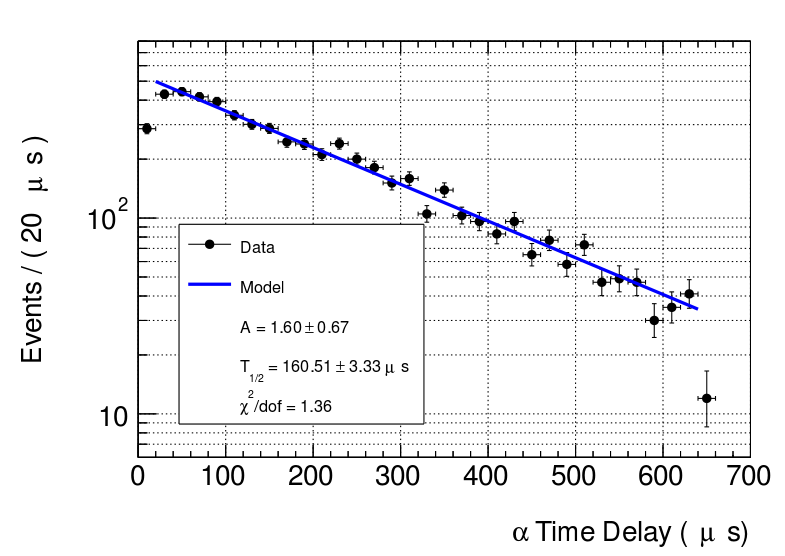
\includegraphics[scale=0.35]{pictures/Chap6/alphaTimeDelay1e1aChannel.png}
\label{1e1aChannel_alphaDelayTime}
\caption{Average time delay between the electron and the $\alpha$ candidate Geiger hits in 1e1$\alpha$ channel. The blue line is an exponential fit which matches to the $^{\text{214}}$Bi half-life.}
\end{figure}


\begin{table}
\centering
\begin{tabular}{cc|c}
                    &            &  $^{\text{214}}$Bi Activity (mBq) \\
\midrule
\multirow{2}{*}{P1} & Wire surf. & 667 $\pm$ 27 \\ 
                    & Foil surf. & 15 $\pm$ 1 \\
\midrule
\multirow{2}{*}{P2} & Wire surf. & 91 $\pm$ 5 \\ 
                    & Foil surf. & 1.3 $\pm$ 0.3 \\
\midrule
\multicolumn{2}{c|}{Mylar (mBq/kg)}  & 2.8 $\pm$ 0.2 \\
\midrule
\multicolumn{2}{c|}{Internal (mBq/kg)}  & 0.4 $\pm$ 0.1 \\
\bottomrule
\end{tabular}
\caption{$^{\text{214}}$Bi  activity measured in the \Cd~sector}
\label{Table1e1a-activityMeasurement}
\end{table}

\FloatBarrier


\subsubsection{Internal $^{\text{208}}$Tl ($^{\text{220}}$Rn) measurement}


\NI The $\beta$-decay of $^{\text{208}}$Tl is almost always accompanied by a cascade of photons from the excited states of $^{\text{208}}$Pb as shown in Figure~\ref{Tl208-decay-schema}. To measure the $^{\text{208}}$Tl activity, one of the most sensitive channel is provided by the 1e2$\gamma$ channel defined by : 


\begin{itemize}
\item
\item
\end{itemize}


\NI The best discriminant variable to distinguish between the $^{\text{208}}$Tl contribution from the isotopes which contribute to 1e2$\gamma$ channel is given by the sum of the electrons and photons energies.  Above E$_{\text{Tot}} > $3 MeV, a pure sample of $^{\text{208}}$Tl is obtained, this distribution is used to perform the likelihood fit.


\begin{figure}[h!]
\centering
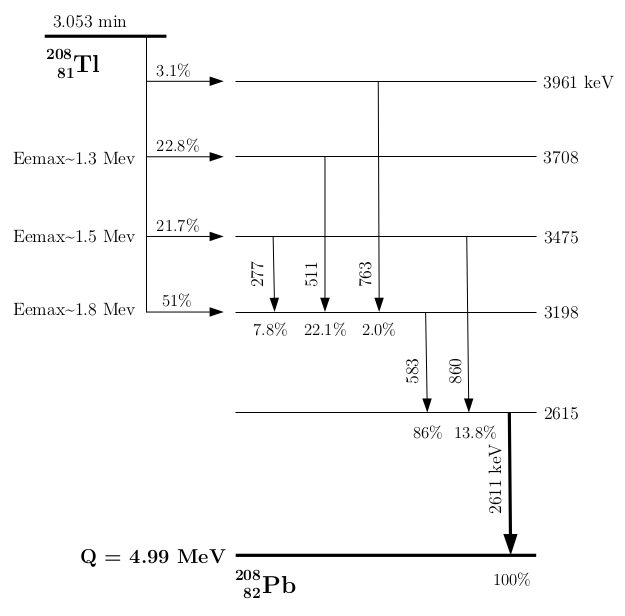
\includegraphics[scale=0.33]{pictures/Chap6/decay-tl208.png}
\caption{Simplified decay diagrams of $^{\text{208}}$Tl.}
\label{Tl208-decay-schema}
\end{figure}


\NI In 1e2$\gamma$ and 1e3$\gamma$, the energies sum of the electrons and photons is used to distinguish between the $^{\text{208}}$Tl contribution and the isotopes which contribute to 1e2$\gamma$ channel. Above E$_{\text{Tot}} > $3 MeV, a pure sample of $^{\text{208}}$Tl is obtained, this distribution is used to perform the likelihood fit.



\begin{figure}[h!]
\centering
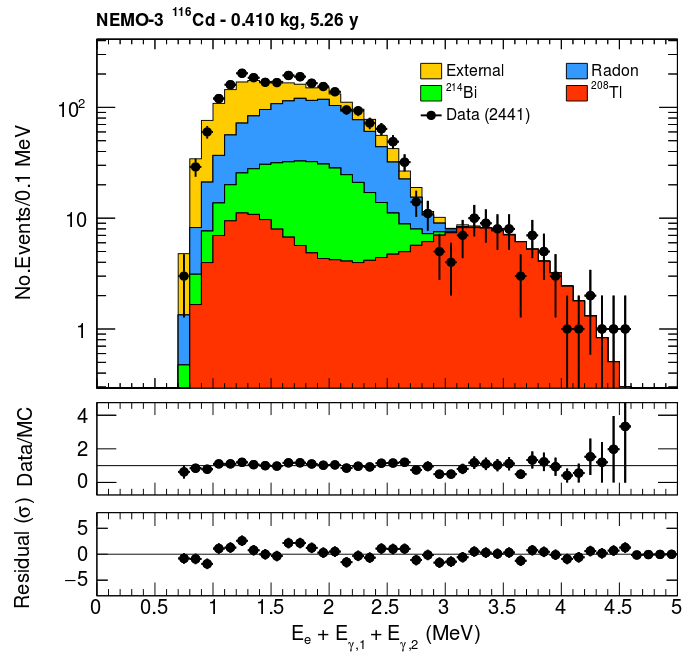
\includegraphics[scale=0.35]{pictures/Chap6/1e2gChannelEtot.png}
\caption{Total energy distribution (E$_e$ + E$_{\gamma_1}$ + E$_{\gamma_2}$) in the 1e2$\gamma$ channel.}
\label{1e2gChannel_Etot}
\end{figure}



\subsubsection{Other internal contributions ($^{\text{40}}$K, $^{\text{234m}}$Pa and $^{\text{210}}$Bi)}\label{sec:1echannel}



\begin{figure}[h!]
\centering
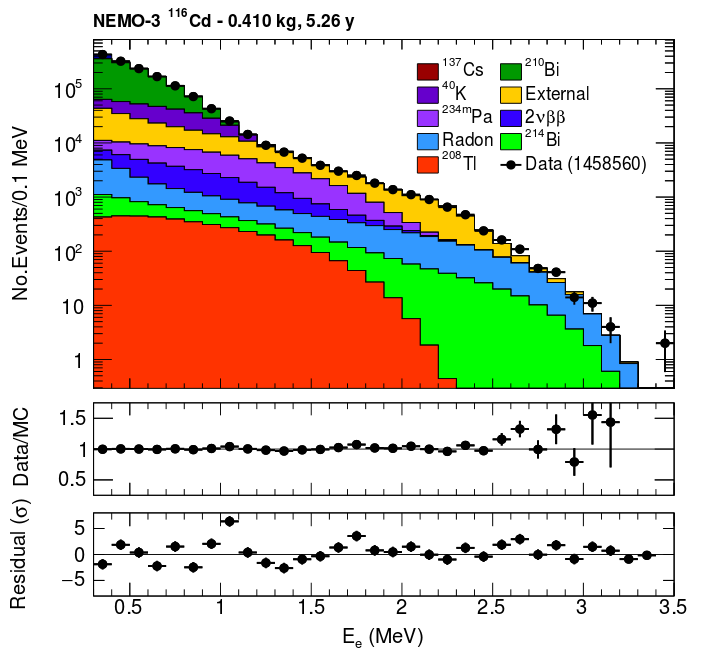
\includegraphics[scale=0.40]{pictures/Chap6/1eChannelEe.png}
\label{1eChannel_Ee}
\caption{Electron energy distribution of the electron in the 1e channel. The three main components are $^{\text{40}}$K, $^{\text{234m}}$Pa and $^{\text{210}}$Bi.}
\end{figure}



\begin{table}
\centering
\begin{tabular}{c|c}
 & Activity (Bq) \\
\midrule
$^{\text{40}}$K                 & 0.0152 $\pm$ 0.0001 \\
$^{\text{234m}}$Pa              & 0.0037 $\pm$ 0.0001 \\
$^{\text{210}}$Bi (surf. foil)  & 3.91   $\pm$ 0.01   \\
$^{\text{210}}$Bi (surf. wire)  & 2.4    $\pm$ 0.1    \\
\bottomrule
\end{tabular}
\caption{Measured activity in 1e channel of the other internal components. }
\label{Table1e-activityMeasurement}
\end{table}



\FloatBarrier




\subsubsection{Background model validation}


\NI The background model is validated by measuring the activity of $^{\text{208}}$Tl and $^{\text{214}}$Bi in the 1e1$\gamma$ channel. The results are then compared to the measurement obtained in 1e1$\alpha$ channel for $^{\text{214}}$Bi and 1e2$\gamma$ and  1e3$\gamma$ channels for $^{\text{208}}$Tl. The very good agreement ($<$ 1 $\sigma$) of the results validates the background model.




The considered channels and the contaminations they can measured are summarized in Table \ref{TableChannelBKG}.  

%The selection criteria of each channel can be found in~\cite{Arnold2016bed}. 


\begin{table}[h!]
\centering
\begin{tabular}{c|c}
\toprule
Contaminations & Channels \\[0.1cm]
\midrule
$^{\text{214}}$Bi,$^{\text{222}}$Rn                    & 1e1$\alpha$                           \\[0.1cm]  
Externals                                              & OCE and ($\gamma$, e)$_{\text{Ext}}$  \\[0.1cm]
$^{\text{208}}$Tl                                      & 1e2$\gamma$  and 1e3$\gamma$          \\[0.1cm]
$^{\text{40}}$K, $^{\text{234m}}$Pa, $^{\text{210}}$Bi & 1e                                    \\[0.1cm]
$^{\text{208}}$Tl,$^{\text{214}}$Bi                    & 1e1$\gamma$                           \\[0.1cm] 
\bottomrule
\end{tabular}
\caption{Contaminations under consideration and channels in which they can be measured.}
\label{TableChannelBKG}
\end{table}




\NI The summary of all the activities measured in all these different channels is shown in Table \ref{SummaryAllActivities}. A total of 26 contributions are taking into account in the background model. The contribution of the $\beta \beta$ decay of \Cd~to the ground state is also added and constitute the 27$^{\text{th}}$ background contributions.



\begin{table}
\centering
\begin{tabular}{c|c|c|c}
 \toprule
 \multicolumn{3}{c|} {}& Activities \\[0.1cm]
 \midrule
 \midrule
 \multirow{18}{*}{Internal Background} &  \multirow{6}{*} {$^{\text{214}}$Bi} & Wire surface (P1)  & [667 $\pm$ 27] mBq\\[0.1cm]
  									   &                                      &  Foil surface (P1) & [15 $\pm$ 1] mBq\\[0.1cm]	
  									   &                                      &  Wire surface (P2) & [91 $\pm$ 5] mBq\\[0.1cm]	
  									   &                                      &  Foil surface (P2) & [1.3 $\pm$ 0.3] mBq\\[0.1cm]	
  									   &                                      &  Mylar             & [2.8 $\pm$ 0.2] mBq/kg\\[0.1cm]	
  									   &                                      &  Internal          & [0.36 $\pm$ 0.1] mBq/kg\\ \cmidrule{2-4}
  									   
   									   &  $^{\text{208}}$Tl                   & Internal           & [0.14 $\pm$ 0.02] mBq/kg \\ \cmidrule{2-4}
   									   
   									   &  \multirow{2}{*}{$^{\text{40}}$K}    & Low           & [0.0054 $\pm$ 0.0001] Bq\\[0.1cm]
   									   &                                & Medium              & [0.0098 $\pm$ 0.0001] Bq\\ \cmidrule{2-4}
   									   
    								   &  \multirow{2}{*}{$^{\text{234m}}$Pa} & Low               & [0.0013 $\pm$ 0.0001] Bq\\[0.1cm]
    								   &                                &  Medium             & [0.0021 $\pm$ 0.0002] Bq\\ \cmidrule{2-4}
    								   
    								   &  \multirow{3}{*}{$^{\text{210}}$Bi}   & Low                 & [1.15 $\pm$ 0.01] Bq\\[0.1cm]
    								   &                                & Medium   			  & [2.76 $\pm$ 0.01] Bq\\[0.1cm]
    								   &                                & Wire Surface        & [2.4 $\pm$ 0.1] Bq\\
    								  
 \midrule
 \multirow{15}{*}{External Background} & \multirow{2}{*} {$^{\text{40}}$K}    & PMT                  & [1300 $\pm$ 45] Bq\\[0.1cm]
  									   &                               &  Scintillator        & [19 $\pm$ 1] Bq\\ \cmidrule{2-4}
  									   	
    								   & \multirow{4}{*} {$^{\text{214}}$Bi}  & PMT                  & [269 $\pm$ 47] Bq\\[0.1cm]
  									   &                               & Air LSM (P1)         & [600 $\pm$ 20] Bq\\  			
   									   &                               & Scintillator         & [0.25 $\pm$ 0.03] Bq\\[0.1cm]
  									   &                               &  Fe Shield           & [10303 $\pm$ 2023] Bq\\ \cmidrule{2-4}    								  
    								   & \multirow{3}{*} {$^{\text{208}}$Tl}  & PMT                  & [45.4 $\pm$ 1.4] Bq\\[0.1cm]
    								   &                               &  Air LSM (P1)        & [14 $\pm$ 3] Bq\\[0.1cm]
     								   &                               &  Fe Shield           & [55 $\pm$ 50] Bq\\ \cmidrule{2-4}  								     									   
    								   & $^{\text{210}}$Bi  		   & Scintillator         & [35 $\pm$ 4] Bq\\ \cmidrule{2-4}
    								   & $^{\text{60}}$Co    		   & Tower $+$ mu metal   & [62 $\pm$ 13] Bq\\ \cmidrule{2-4}
    								   & $^{\text{234m}}$Pa			   & Mu metal             & [2655 $\pm$ 1180] Bq\\ %\cmidrule{2-4}
 \bottomrule
 \bottomrule
\end{tabular}
\caption{Measured activities of each componant of the background model.}
\label{SummaryAllActivities}
\end{table}
 





\FloatBarrier

\section{Events preselection}


The preselection consists of a set of critria to select the events coming from the \Cd~sector and containing 2 electrons and photons. The events with an alpha particle are not selected.

\bigskip 

\NI An electron is defined as a particle having a negative track with a vertex on the source foil and hitting a calorimeter. In a first time, the energy of each electron has to be greater than 300~keV and the minimal length of their track is 50~cm.
\noindent A photon is defined as calorimeter hit no associated to a track. To avoid calorimeter noise the energy of the photon has to be greater than 150~keV.
\noindent An alpha particle is identified as a delayed hits inside the tracker volume. Others criteria as the status of the PMT, or the internal/probability of the electrons are added. The complete list of the preselectrion criteria can be found below :


\begin{itemize}
\item
\item
\end{itemize}



\NI This preselection is applied on all the MC of excited states and all the background componants. It consists of the first step of the selection which is common to all the excited states. Latter, other cuts will be added to optimize the background rejection according the excited state studied.


\subsection{Signal efficiency}


\NI From the MC, the signal efficiency of each excited state can be computed by comparing the number of events which passes the preselection to the number of generated events. The results are given in Table \ref{EffPreselection}. 


\bigskip


\begin{table}[h!]
\begin{center}
\begin{tabular}{c|c|c|c}
\toprule
Excited state & N$_\text{{generated}}$ & N$_\text{{preselected}}$ & $\epsilon_\text{{preselection}}$ \\[0.1cm]
\midrule
(0$^+$) 2$\nu$ & 200 000 000 & 11168 & (5.58~$\pm$~0.05)~10$^{-\text{5}}$\\[0.1cm]
(0$^+$) 0$\nu$ &   4 999 900 & 17681 & (3.54~$\pm$~0.03)~10$^{-\text{3}}$\\[0.1cm]
(2$^+$) 2$\nu$ &  10 000 000 & 13095 & (1.31~$\pm$~0.01)~10$^{-\text{3}}$\\[0.1cm]
(2$^+$) 0$\nu$ &   5 000 000 & 91165 & (1.82~$\pm$~0.01)~10$^{-\text{2}}$\\[0.1cm]
\bottomrule
\end{tabular}
\caption{Signal efficiency of the preselection 2eN$\gamma$ of each excited states.}
\label{EffPreselection}
\end{center}
\end{table}


\subsection{Number of expected background}
\subsection{2e1$\gamma$ channel}
\subsection{2e2$\gamma$ channel}

\section{Cut optimisation using multi-approach}

\section{Systematics uncertainties}

\section{$\beta\beta$ decay rate of $^{\text{116}}$Cd into the excited states of $^{\text{116}}$Sn}


\end{document}